\chapter{Result analysis and discussion}


\section{Experimental setup}
All models were trained using the PyTorch framework on a GPU-enabled environment. MobileNetV2 and ShuffleNetV were trained for 20 epochs, while ResNet18 was trained for 10 epochs due to faster convergence. For optimization, MobileNetV2 and ResNet18 were trained using the Adam optimizer, while ShuffleNet employed AdamW to enhance generalization performance. Learning rates were set to 0.001 for MobileNetV2 and ShuffleNet, and 0.0001 for ResNet18 to ensure stable training. All models were trained with a batch size of 32 and an input image resolution of 224 × 224. Cross-entropy loss was used as the optimization objective. Data augmentation techniques such as horizontal flipping and rotation were applied to improve model robustness.
\begin{table}[H]

\label{tab:mobilenet_params}
\begin{tabular}{ll}
\toprule
\textbf{Parameter} & \textbf{Value} \\
\midrule
Model & MobileNetV2 \\
Optimizer & Adam \\
Learning Rate & 0.001 \\
Batch Size & 32 \\
Epochs & 20 \\
Input Size & 224 $\times$ 224 \\
Number of Classes & 5 \\
Loss Function & Cross-Entropy Loss \\
Data Augmentation & Horizontal Flip, Rotation (10$^\circ$), Normalization \\
\bottomrule
\end{tabular}
\centering
\caption{Training Parameters for MobileNetV2}
\end{table}

\begin{table}[H]

\label{tab:shufflenet_params}
\begin{tabular}{ll}
\toprule
\textbf{Parameter} & \textbf{Value} \\
\midrule
Model & ShuffleNetV2 \\
Optimizer & AdamW \\
Learning Rate & 0.001 \\
Batch Size & 32 \\
Epochs & 20 \\
Input Size & 224 $\times$ 224 \\
Number of Classes & 5 \\
Loss Function & Cross-Entropy Loss \\
Scheduler & ReduceLROnPlateau (patience = 3) \\
Data Augmentation & Resize, Grayscale $\rightarrow$ RGB, Random transforms \\
\bottomrule
\end{tabular}
\centering
\caption{Training Parameters for ShuffleNet}
\end{table}


\begin{table}[H]

\label{tab:resnet_params}
\begin{tabular}{ll}
\toprule
\textbf{Parameter} & \textbf{Value} \\
\midrule
Model & ResNet18 \\
Optimizer & Adam \\
Learning Rate & 0.0001 \\
Batch Size & 32 \\
Epochs & 10 \\
Input Size & 224 $\times$ 224 \\
Number of Classes & 5 \\
Loss Function & Cross-Entropy Loss \\
Data Augmentation & Normalization only with flip or rotation\\
\bottomrule
\end{tabular}
\centering
\caption{Training Parameters for ResNet18}
\end{table}

\section{Training Performance analysis}

\subsection{Training overview for Mobilnet V2}

\begin{figure}[h]
    \centering
    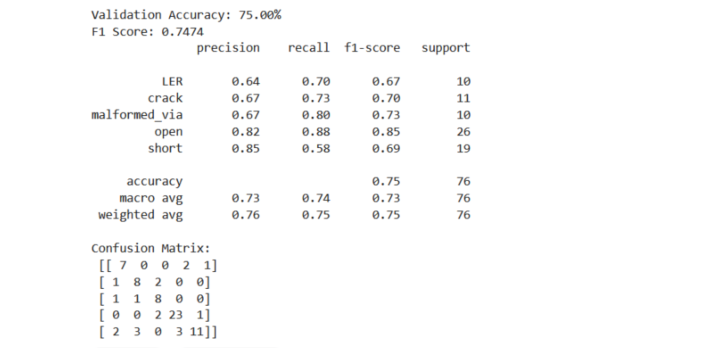
\includegraphics[width=0.8\textwidth]{Images_And_Tables/MobilNetV2_Training.png}
    \caption{MobilnetV2 Training Overview}
    \label{fig:MobilnetV2_Training_Overview}
\end{figure}

\subsubsection{Observation}
An accuracy of approximately 75\% is considered acceptable in this context, given the use of MobileNetV2, which prioritizes computational efficiency over representational complexity for edge deployment. The application of INT8 quantization further reduces numerical precision, contributing to a slight drop in accuracy. Considering the inherent complexity of SEM images and the limited computational capabilities of the Raspberry Pi platform, this result reflects a practical balance between predictive performance and real-time execution constraints.


\subsection{Training overview for Shufflenet}

\begin{figure}[H]
    \centering
    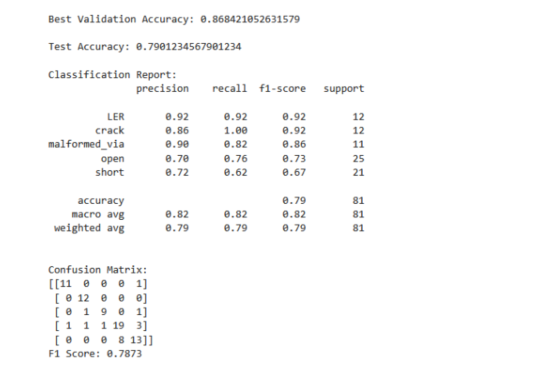
\includegraphics[width=0.8\textwidth]{Images_And_Tables/ShuffleNet_Training.png}
    \caption{ShuffleNet Training Overview}
    \label{fig:ShuffleNet_Training_Overview}
\end{figure}
\subsubsection{Observation}
The ShuffleNet model attained an accuracy of approximately 76\%, along with an F1-score of 0.75, indicating a balanced performance across the evaluated classes.
 This is expected given its lightweight architecture, which prioritizes computational efficiency using grouped and depthwise convolutions. The confusion matrix indicates that some defect classes are misclassified due to visual similarity and limited feature representation. However, the model offers significant advantages in terms of low latency and small model size, making it highly suitable for deployment on resource-constrained edge devices like Raspberry Pi


\subsection{Training overview for Resnet18}
\begin{figure}[H]
    \centering
    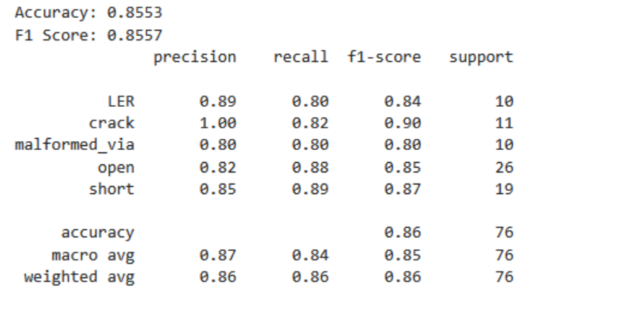
\includegraphics[width=0.8\textwidth]{Images_And_Tables/ResNet18.png}
    \caption{ResNet18 Training Overview}
    \label{fig:ResNet18_Training_Overview}
\end{figure}

\subsubsection{Observation}
Among the evaluated models, ResNet18 achieved the highest accuracy of approximately 85.5\%, that can be attributed to its deeper network structure and the use of residual connections that enable more effective feature learning. However, this improved performance comes at the cost of increased computational complexity, making it less suitable for real-time deployment on resource-constrained edge devices. As a result, ResNet18 is primarily used as a reference model, while lightweight architectures are preferred for practical edge-based implementation.


\section{Edge inference result over Raspberry Pi4}

\subsection{Edge inference result for MobilNetV2}
\begin{figure}[H]
    \centering
    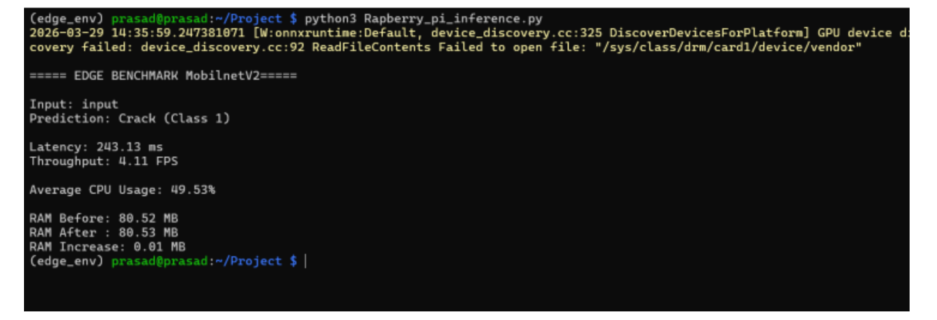
\includegraphics[width=0.8\textwidth]{Images_And_Tables/MobilNetV2_Edge_Inference.png}
    \caption{Edge inference result for MobilNetV2}
    \label{fig:MobilNetV2_Edge_Inference}
\end{figure}


\subsection{Edge inference result for ShuffleNet}
\begin{figure}[H]
    \centering
    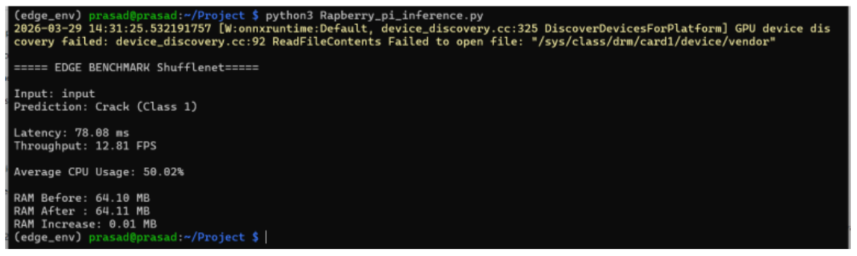
\includegraphics[width=0.8\textwidth]{Images_And_Tables/ShuffleNet_Edge_Inference.png}
    \caption{Edge inference result for ShuffleNet}
    \label{fig:ShuffleNet_Edge_Inference}
\end{figure}

\subsection{Edge inference result for ResNet18}
\begin{figure}[H]
    \centering
    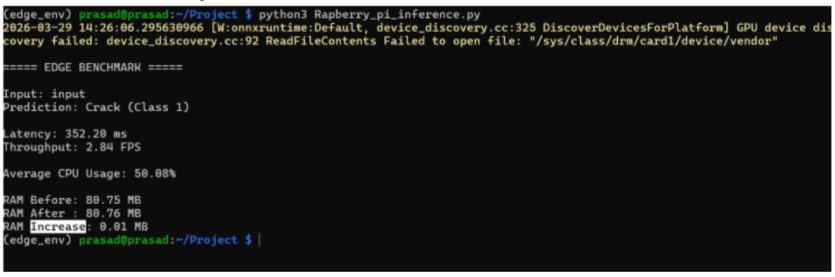
\includegraphics[width=0.8\textwidth]{Images_And_Tables/ResNet18_Edge_Inference.png}
    \caption{Edge inference result for ResNet18}
    \label{fig:ResNet18_Edge_Inference}
\end{figure}

\subsection {Quantitative Model Comparison}

Add Edge Deployment Results \& Comparison table


% Table 1 : Classification Performance
\begin{table}[htbp]
\centering

\footnotesize
\renewcommand{\arraystretch}{1.3}
\setlength{\tabcolsep}{5pt}

\begin{tabular}{|c|c|c|c|c|c|}
\hline
\multicolumn{6}{|c|}{\textbf{Classification Performance}} \\
\hline

\rowcolor{yellow}
\textbf{Sl.No} &
\textbf{Model} &
\textbf{Overall Accuracy} &
\textbf{F1 Score} &
\makecell{\textbf{Model Size in MB} \\ \textbf{After Quantization}} &
\makecell{\textbf{Latency in ms} \\ \textbf{(Kaggle)}} \\
\hline

1 & MobileNetV2 & 0.7530 & 0.7400 & 2.23 & 99.53 \\
\hline
2 & ShuffleNet  & 0.7600 & 0.7594 & 1.30 & 28.19 \\
\hline
3 & ResNet18    & 0.8024 & 0.8552 & 10.70 & 128.71 \\
\hline

\end{tabular}
\caption{Classification Performance of Selected Models}
\label{tab:classification_performance}
\end{table}

% Table 2 : Edge Inference Performance
\begin{table}[htbp]
\centering

\scriptsize
\renewcommand{\arraystretch}{1.3}
\setlength{\tabcolsep}{5pt}

\begin{tabular}{|c|c|c|c|c|c|c|}
\hline
\multicolumn{7}{|c|}{\textbf{Edge Inference Performance}} \\
\hline

\rowcolor{yellow}
\textbf{Sl.No} &
\textbf{Model} &
\textbf{Edge Suitability} &
\textbf{Edge Latency (ms)} &
\textbf{Throughput} &
\makecell{\textbf{Average CPU} \\ \textbf{Usage}} &
\textbf{RAM Increase} \\
\hline

1 & MobileNetV2 & Good      & 244.98 & 4.08  & 49.44 & 0.01 \\
\hline
2 & ShuffleNet  & Excellent & 78.08  & 12.81 & 50.02 & 0.01 \\
\hline
3 & ResNet18    & Poor      & 352.20 & 2.84  & 50.08 & 0.01 \\
\hline

\end{tabular}
\caption{Edge Inference Performance of Selected Models}
\label{tab:edge_inference_performance}
\end{table}

\section{Grad-CAM Qualitative and quantitative analysis}
The model concentrated strongly on the fracture region, indicating that prediction was based on relevant structural discontinuity.

Keep the table for IOU and activation ratio


\begin{table}[htbp]
\centering

\renewcommand{\arraystretch}{1.3}

\begin{tabular}{|c|c|c|c|}
\hline
\rowcolor{yellow}
\textbf{SL. No} & \textbf{Model Used} & \textbf{Mean IOU} & \textbf{Activation Ratio} \\

\hline
1 & ShuffleNet   & 0.2800 & 0.8140 \\
\hline
2 & MobileNetV2  & 0.3135 & 0.8153 \\
\hline
3 & ResNet18     & 0.3576 & 0.8230 \\
\hline

\end{tabular}
\caption{Quantitative Grad-CAM Comparison of Selected Models}
\label{tab:gradcam_comparison}
\end{table}

\subsection{Grad-CAM visualization for MobilenetV2}
\begin{figure}[H]
    \centering
    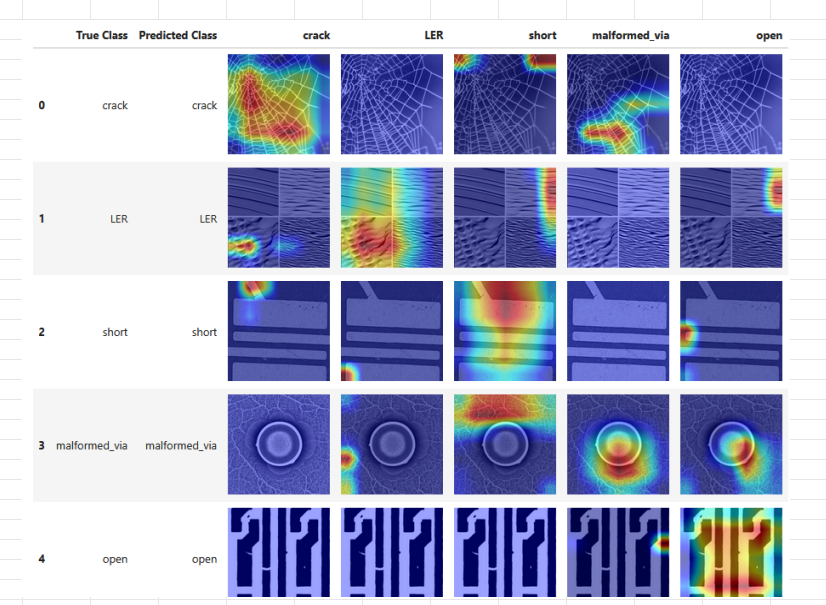
\includegraphics[width=0.6\textwidth]{Images_And_Tables/MobilNet_V2_Grad-Cam.png}
    \caption{Grad-Cam over MobilNetV2}
    \label{fig:Grad-Cam over MobilNetV2}
\end{figure}

\subsection{Grad-CAM visualization for ShuffleNet}
\begin{figure}[H]
    \centering
    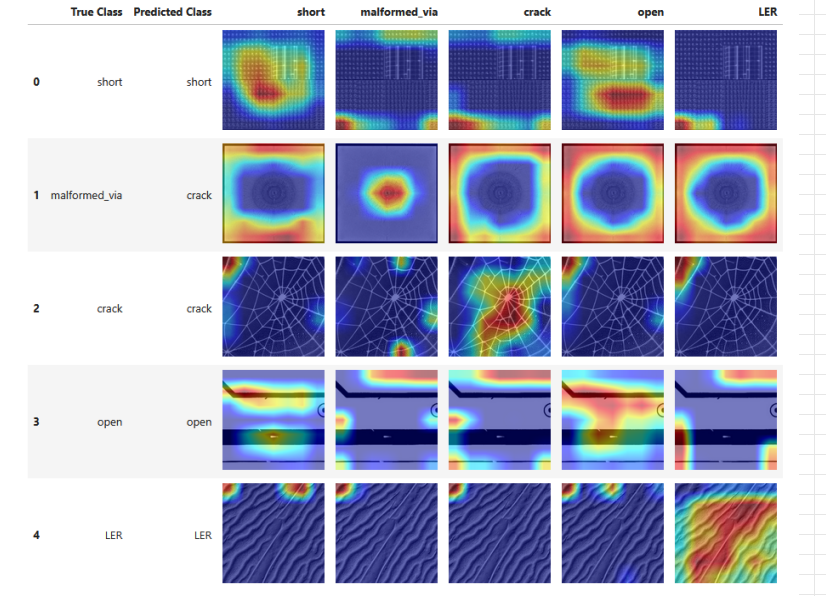
\includegraphics[width=0.6\textwidth]{Images_And_Tables/ShuffleNet_Grad-cam.png}
    \caption{Grad-Cam over ShuffleNet }
    \label{fig:Grad-Cam over ShuffleNet}
\end{figure}

\subsection{Grad-CAM visualization for ResNet18}
\begin{figure}[H]
    \centering
    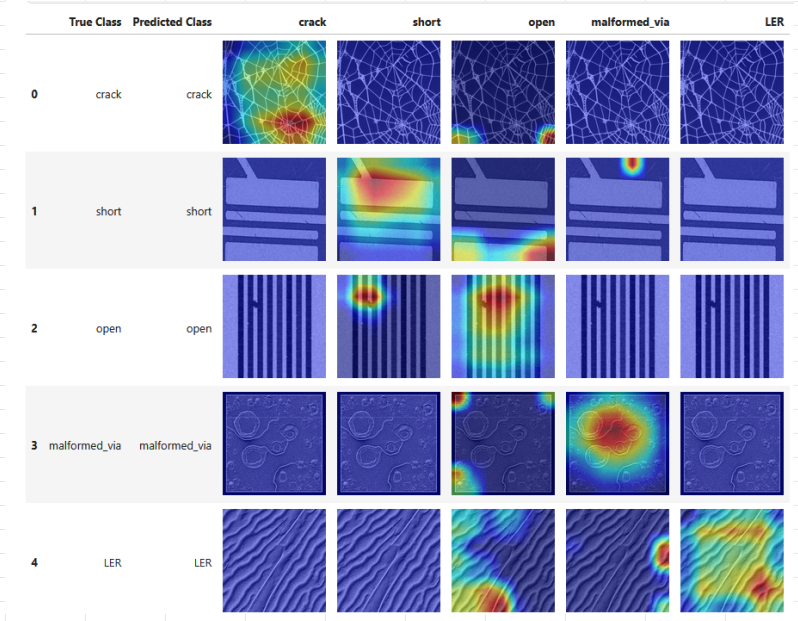
\includegraphics[width=0.6\textwidth]{Images_And_Tables/ReseNet18_Grad-Cam.png}
    \caption{Grad-Cam over ResNet18 }
    \label{fig:Grad-Cam over ResNet18}
\end{figure}

\section{Observations \& Reasoning:}


\subsection{Correlation Between Classification Performance and Localization}

\subsubsection{Observation}
\begin{itemize}
\item Models with higher Accuracy and F1-score (e.g., ResNet18) also exhibit higher Mean IoU and better Grad-CAM activation alignment.
\item Lower-performing models (e.g., ShuffleNet) show both reduced classification metrics and weaker localization.
\end{itemize}

\subsubsection{Reasoning}
\begin{itemize}

\item High classification performance indicates that the model has learned discriminative features, which also improves its ability to focus on relevant spatial regions.
\item Grad-CAM confirms that correct predictions are associated with focused and meaningful activation maps.
\end{itemize}

\subsection{ResNet18 – High Accuracy, Strong Localization, Higher Cost}
\subsubsection{Observation}
\begin{itemize}
\item High classification performance indicates that the model has learned discriminative features, which also improves its ability to focus on relevant spatial regions.
\item Grad-CAM shows precise and concentrated attention on defect regions
\item Larger model size and relatively higher inference time
\end{itemize}


\subsubsection{Reasoning}
\begin{itemize}

\item Residual connections enable deeper feature learning without degradation
\item Captures both low-level textures and high-level semantics \&
Produces highly discriminative and spatially aligned features
\end{itemize}

\subsection{MobileNetV2 – Balanced Trade-off}
\subsubsection{Observation}
\begin{itemize}
\item Slightly lower Accuracy and F1-score than ResNet18 \&
Moderate Mean IoU
\item Grad-CAM shows reasonably correct but slightly diffused attention
\item Significantly smaller model size and faster inference
\end{itemize}


\subsubsection{Reasoning}
\begin{itemize}

\item Depthwise separable convolutions reduce computation
\item Some spatial detail is lost due to compression
\item Leads to moderate localization precision
\end{itemize}

\subsection{ShuffleNet – Efficient but Limited Learning Capacity}
\subsubsection{Observation}
\begin{itemize}
\item Lowest Accuracy and F1-score \& Lowest Mean IoU
\item Grad-CAM heatmaps are diffused and occasionally misaligned
\item Smallest model size and fastest inference
\end{itemize}


\subsubsection{Reasoning}
\begin{itemize}

\item Channel shuffling and grouped convolutions limit feature interaction

\item Reduced representational capacity affects fine-grained defect detection

\end{itemize}

\subsection{Edge Deployment Trade-off Analysis}
\subsubsection{Observation}
\begin{itemize}
\item ResNet18 - Best accuracy \& localization but higher latency
\item MobileNetV2 - Balanced performance and speed
\item ShuffleNet - Fastest but least reliable
\end{itemize}


\subsubsection{Reasoning}
\begin{itemize}

\item Edge systems require low latency and low memory usage

\item However, poor localization (as seen in Grad-CAM) may lead to incorrect inspection decisions

\end{itemize}


\subsection{Grad-CAM Analysis for Correct and Incorrect Predictions}
\subsubsection{Observation}
\begin{itemize}
\item High-performing models show strong activation in defect regions \& Minimal background interference
\item Moderately performing models show Activation shifts to non-defect regions \& Heatmaps become diffused or fragmented
\end{itemize}


\subsubsection{Reasoning}
\begin{itemize}

\item High performing models indicate successful learning of relevant spatial features

\item Model confusion due to similar texture, limited resolution

\item Grad-CAM analysis confirms that misclassifications are strongly associated with incorrect spatial attention, emphasizing the importance of interpretability in evaluating model reliability

\end{itemize}

\subsection{Final comparative insight}
\subsubsection{Observation}
\begin{itemize}
\item High accuracy is not always best for deployment
\item Fast models are not always reliable
\end{itemize}


\subsubsection{Reasoning}
\begin{itemize}

\item Deployment decision must consider Accuracy, Localization, inference time and model size

\item While ResNet18 delivers superior classification and localization performance, MobileNetV2 offers a more practical balance for edge deployment. ShuffleNet, despite its efficiency, may not be suitable for critical defect inspection tasks due to its limited localization capability

\end{itemize}